%%%%%%%%%%%%%%%%%%%%%%%%%%%%%%%%%%%%%%%%%%%%%%%%%%%%%%%%%%%%%%%%%%%%%%%%%%%%%%%%%%
%%													
							%%
%% File name: 		20hannes.tex									
			%%
%% Project name:	Hochleistungsantenne								
		%%
%% Type of work:	T3X00 project work								
			%%
%% Author:			Sarah Brückner, Maximilian Stiefel, Hannes Bohnengel		%%
%% Date:			30th May 2016								
				%%
%% University:		DHBW Ravensburg Campus Friedrichshafen						
%%
%% Comments:		Created in gedit with tab width = 4						
	%%
%%													
							%%
%%%%%%%%%%%%%%%%%%%%%%%%%%%%%%%%%%%%%%%%%%%%%%%%%%%%%%%%%%%%%%%%%%%%%%%%%%%%%%%%%%


\chapter{Aufbau der Bodenstation}
\label{chap:bodenstation}
Die Bodenstation mit oder über Satelliten der DHBW Ravensburg am Standort Friedrichshafen besteht grundsätzlich aus folgenden 
Komponenten:
\section{Antennen}
\begin{figure}
  \centering
	\begin{minipage}[t]{0.3\textwidth}
		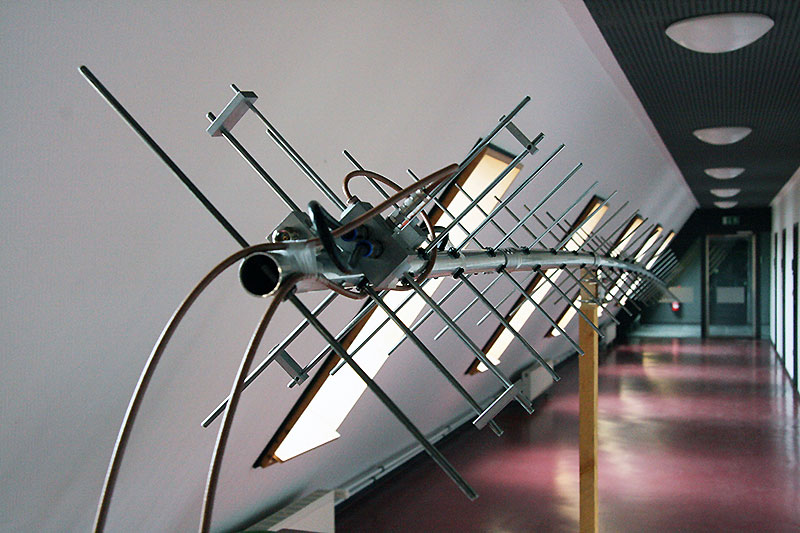
\includegraphics[width=\textwidth]{images/antenne}
	\end{minipage}
	\begin{minipage}[t]{0.3\textwidth}
		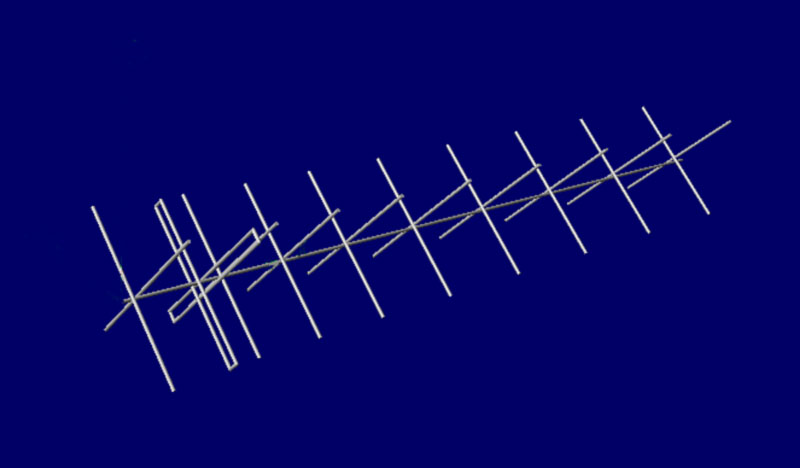
\includegraphics[width=\textwidth]{images/antenne2}
	\end{minipage}
	\begin{minipage}[t]{0.2\textwidth}
		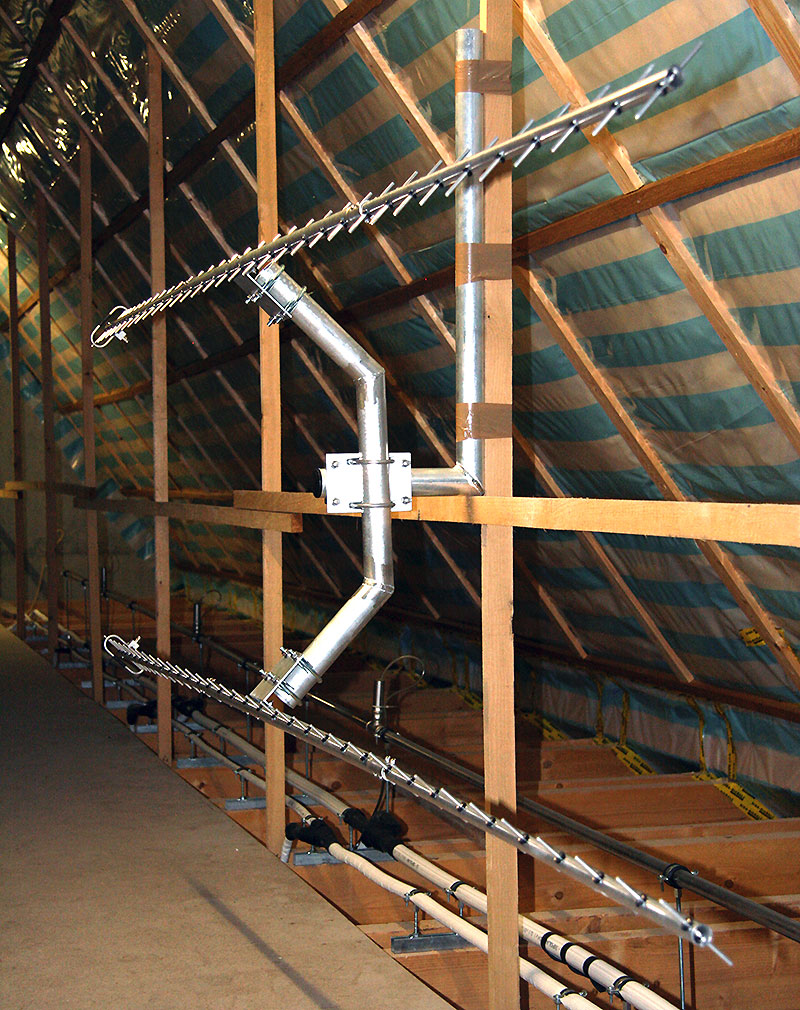
\includegraphics[width=\textwidth]{images/antenne3}
	\end{minipage}
	\caption[Antennen]{436CP42UG 70-cm, WX220 2-m und 23CM35 23-cm, Quelle: \cite{dk0te}}
	\label{fig: antennen}
\end{figure}
In der unteren Grafik ist von links nach rechts eine Kreuzyagi-Antenne für das 70-cm-Band, eine Kreuzyagi-Antenne für das 2-m-Band und eine 
Yagiantenne für das 23-cm-Band zu sehen. Dazu gehören ein Mast sowie Vorverstärker und Polarisationsschalter. Die Yagiantennen für das 23- und 
70-cm-Band kommen von der Firma M$^2$ und die Kreuzyagi-Antenne von der Firma WIMO. Yagiantennen bestehen aus einem Faltdipol, einem Reflektor und 
mehreren Direktoren. Aus der Vorlesung Hochfrequenztechnik \cite{hfscript} ist bekannt, dass ein Reflektor ca. 5 $\%$ länger als $\frac{\lambda}{2}$ 
ist, somit oberhalb seiner Resonanzfrequenz betrieben wird und daher induktiv wirkt.  Anders ist es beim Direktor. Dieser wird von Direktor zu 
Direktor um ca. 5 $\%$ kürzer und wird im unteren Resonanzfrequenzbereich betrieben. Der Reflektor erhöht den Antennengewinn durch Reflexion der 
einfallenden Wellen auf dem Dipol. Die Direktoren beeinflussen die Abstrahlcharakteristik der Antenne, da die keulenförmige Ausprägung stärker wird.  
Durch die kreuzförmige Aneinanderreihung der Kreuzyagi-Antenne können Funkwellen mit horizontaler und vertikaler Polarisation empfangen werden. Bei 
der linken Kreuzyagi-Antenne sieht man in der Grafik den Reflektor und dahinter, den Faltdipol. Darauf folgen die Direktoren. Folgende 
Antennengewinne werden von den Antennen bereitgestellt: 436CP42UG (70-cm): 18.90 dBic, 23CM35 (23-cm): 20.94 dBi und WX220 (2-m): 35.00 dBi.
\clearpage

\section{Rotoren}
Um die Yagiantennen steuern zu können werden Rotoren sowie dessen Steuergeräte von der Bodenstation zur Verfügung gestellt.
\begin{figure}[h]
 \centering
 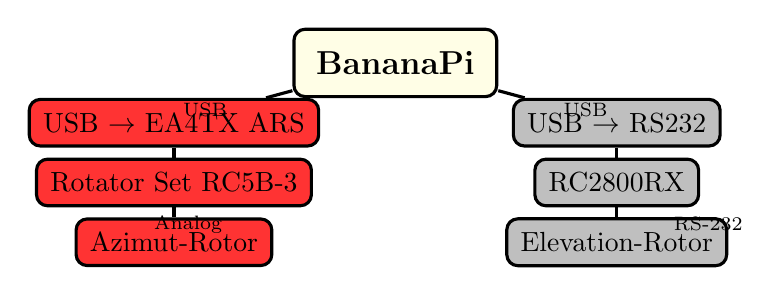
\begin{tikzpicture}[every node/.style = {shape=rectangle, rounded corners, draw, align=center, scale=1}, line width=0.4mm, level 
distance=1.8\baselineskip, level 1/.style = {sibling distance=16em}, level 2/.style = {sibling distance=8em}]
	\tikzstyle{top} = [fill=yellow!10, inner sep=8pt, font=\bfseries\large]
	\tikzstyle{az} = [fill=red!80, inner sep=5pt]
	\tikzstyle{el} = [fill=gray!50, inner sep=5pt]
	\tikzstyle{label} = [draw=none, font=\scriptsize, right]
	\node[top]{BananaPi}
	child { node[az]{USB $\rightarrow$ EA4TX ARS} 
		child { node[az]{Rotator Set RC5B-3} 
		  child { node[az]{Azimut-Rotor} } } }
	child { node[el]{USB $\rightarrow$ RS232}
		child { node[el]{RC2800RX}
		  child { node[el]{Elevation-Rotor} } } };
	\node[label] at (2,-0.6) {USB};
	\node[label,left] at (-2,-0.6) {USB};
	\node[label] at (-3.2,-2.05) {Analog};
	\node[label] at (3.4,-2.05) {RS-232};
% 	\node[label] at (-3.2,-3.5) {};
% 	\node[label] at (3.4,-3.5) {};
\end{tikzpicture} 

 \caption{Rotatorsteuerung}
 \label{fig:azel}
\end{figure}\\
In dem Organigramm \ref{fig:azel} stellt der BananaPi, ein Einplatinencomputer, die Rotorsteuerung als Einheit in dem DHBW Netzwerk bereit. Über die 
ARSVCOM Schnittstelle kann auf ihn zugegriffen werden. %Ref zu Hannes
Über USB sind die Steuergeräte für den Azimut- und Eleavtions-Rotor an den BananaPi angeschlossen. Das Steuegerät RC2800PXEL für den Elevationsrotor 
von der Firma M$^2$ arbeitet mit der seriellen Schnittstelle RS-232. Daher wird ein USB $\rightarrow$ RS232 Adapter benötigt. Um die digitalen 
Kommados des ARS Protokolls umsetzten zu können, benötigt das analoge Steuergerät RC5B-3-P von Create für den Azimutrotor einen Umsetzer von dem 
digitalen in den analogen Bereich. Dies geschieht über das Antennen-Rotor System ARS-USB von EA4TX. In der Grafik \ref{fig:rot} sind die Steuergeräte 
zu sehen.
\begin{figure}[h]
 \centering
 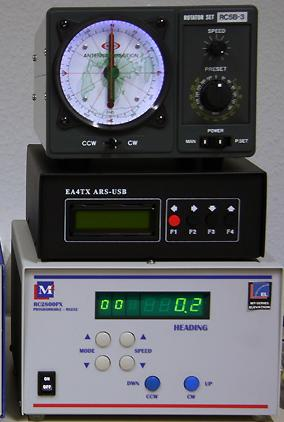
\includegraphics[width=0.225\textwidth]{images/sat-rotor-steuerungen}
 \caption{Steuergeräte für die Rotorsteuerung}
 \label{fig:rot}
\end{figure}
\clearpage

\section{Funkgerät ICOM IC-9100}


% 	\item Funkgerät Icom IC-9100
% 	\begin{itemize}
% 		\item Netcom (2x Seriell zu Ethernet)
% 		\item Netcom Manager Software
% 		\item Hardware für Sprechfunk ?!
% 	\end{itemize}
% \end{itemize}

 
